Das Bedrohungsmodel des theoretisch idealen Mix-Zone Konzeptes \cite{Beresford2003} geht davon aus, dass der Benutzer eines LBS diesem nicht traut. Um aber diesen Service dennoch in Anspruch zu nehmen,  bedient er sich eines Middleware Systems, welches als Proxy zwischen dem Nutzer und dem LBS dient. Das Middleware System unterstützt ihn dabei, seine Identität zu verstecken, indem der Nutzer nur Service Callbacks über das Middleware System und in bestimmten dafür definierten Bereichen empfängt. Dafür meldet der Nutzer Interesse an für ihn relevante LBS bei der Middleware an und diese prüft periodisch den Ort des Nutzers und bestimmt, ob für den Nutzer ein relevantes Event ausgelöst worden ist und reicht ihm die Callbacks zu angemessenen Zeitpunkten weiter. Der Middleware Proxy benutzt Pseudonyme um die Identität des Nutzers vor dem Service zu verstecken.

Da Langzeitpseudonyme es ermöglichen, die Identität des Nutzer über spezifisches Verhalten, wie das Aufhalten an bestimmten Orten wie Zuhause oder auf Arbeit, zu ermitteln, schlägt \cite{Beresford2003} einen ständigen Pseudonymwechsel vor, auch wenn der Nutzer getrackt wird. Die Middleware versorgt den Nutzer regelmäßig mit neuen, unbenutzten Pseudonymen für jede ortssensible Anwendung. Dieser Pseudonymwechsel findet innerhalb der sogenannten Mix-Zone statt. Allerdings können nur LBS genutzt werden, die Pseudonyme unterstützen.

Das Konzept der Mix-Zone wird aus dem Konzept der Mix-Nodes aus dem Bereich der anonymen Kommunikationssystemen abgeleitet \cite{Chow2011}. Die Idee, die hinter dem Mix-Node liegt ist, dass er wartet bis er k Pakete mit gleicher Länge empfangen hat und diese, bevor er sie weiter leitet, zufällig oder nach einer Metrik neu sortiert, so dass eine Unverknüpfbarkeit zwischen eingehenden und ausgehenden Paketen  entsteht.

\cite{Beresford2003} definiert eine Mix-Zone für eine Nutzergruppe als eine zusammenhängende Region mit maximaler Größe, in der keiner dieser Benutzer den Callback eines LBS erhalten hat. Für diese Nutzergruppe können mehrere unterschiedliche Mix-Zones bestehen. Das Gegenstück zu einer Mix-Zone ist die Application Zone, als Gebiet, in der ein Nutzer einen Callback empfangen hat. Der Middleware Proxy kann die Mix-Zones im Voraus oder für jede Nutzergruppe einzeln als Gebiet festlegen, in dem sich gerade kein Stück einer Application Zone befindet.

Weil standortbasierte Anwendungen in Mix-Zones keine ortsbezogenen Informationen erhalten, können sie Benutzer innerhalb der Mix-Zone nicht unterscheiden. Und so kann eine Mix-Zone die Unverknüpfbarkeit zwischen eingehenden und ausgehenden Nutzern erreichen.

\begin{figure}[!h]
		\centering
		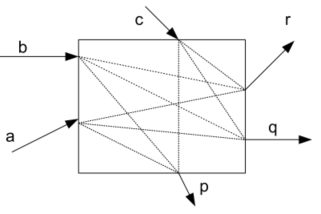
\includegraphics[width=0.5\textwidth]{Bilder/MixZone.PNG}
		\caption{Mix-Zone Model, Quelle: \protect\cite{Palanisamy2011}}
		\label{fig_Palanisamy2011}
\end{figure}

\cite{Palanisamy2011} definiert das eine Mix-Zone Z k-anonymisierend für eine Menge von Nutzern A ist wenn folgende Bedingungen erfüllt sind:
\begin{enumerate}
\item Die Menge A hat mindestens k Elemente, $ |A| \geq k $.
\item Alle Nutzer in A müssen die Mix-Zone Z betreten haben, bevor ein Nutzer aus A die Mix-Zone Z verlässt.
\item Jeder Nutzer der Menge A die Mix-Zone durch einen Eintrittspunkt betritt $ e_{i} \in E $ und diese durch einen Austrittspunkt $ o_{i} \in O $ verlässt und dabei eine zufällige Zeitspanne in der Zone verweilt.
\item Die Übergangswahrscheinlichkeit von jeden Eintrittspunkt zu jeden Austrittspunkt folgt einer Gleichverteilung.
\end{enumerate}